\documentclass[12pt]{article}
\usepackage[utf8]{inputenc} % Sin el guion
\usepackage[T1]{fontenc}    % Ayuda a que las tildes se copien bien del PDF
\usepackage[spanish]{babel}
\usepackage{amsmath}
\usepackage{amssymb}
\usepackage{geometry}
\usepackage[backend=biber,style=numeric]{biblatex}
\usepackage{csquotes}
\usepackage[table,xcdraw]{xcolor} 
\usepackage{tabularx}
\bibliography{referencias}
\geometry{margin=1in}
\usepackage{listings}
\usepackage{xcolor}
\usepackage{xurl}
\usepackage{subcaption}

\usepackage{array}
\usepackage{graphicx}
\usepackage{float}      % opcional, para usar [H]
\usepackage{hyperref}   % opcional, para referencias clickeables

\lstset{
    language=Python,
    basicstyle=\ttfamily\footnotesize,
    keywordstyle=\color{blue},
    commentstyle=\color{gray},
    stringstyle=\color{black},
    numbers=left,
    numberstyle=\tiny,
    frame=single,
    rulecolor=\color{black},
    breaklines=true,
    showstringspaces=false
}

\title{Reto 2: Análisis de Datos con Python \\(Datos Criminalidad en la Ciudad de Montreal)}
\author{Ing. Isaias Garcia Zanella}
\date{\today}

\begin{document}

\maketitle

\section{Introducción}

El análisis de datos criminales representa una herramienta fundamental para comprender los patrones de comportamiento delictivo dentro de una ciudad. Mediante técnicas de análisis exploratorio de datos y visualización geoespacial, es posible identificar tendencias, zonas con alta incidencia criminal y factores temporales asociados a la ocurrencia de delitos.

En el presente proyecto se realizó un análisis de criminalidad de la ciudad de Montreal utilizando herramientas de ciencia de datos en Python. El conjunto de datos empleado contiene información sobre distintos incidentes criminales registrados entre los años 2015 y 2023, incluyendo variables geográficas, temporales y categóricas relacionadas con los delitos reportados.

El objetivo principal del proyecto consistió en responder diferentes preguntas de análisis descriptivo relacionadas con la distribución de los crímenes en la ciudad, los horarios de mayor incidencia, los sectores policiales con mayor actividad delictiva y los tipos de delitos predominantes dentro de cada zona. Para ello, se utilizaron técnicas de limpieza, transformación y visualización de datos mediante librerías especializadas como Pandas, GeoPandas, Matplotlib, Seaborn y Folium.

Adicionalmente, se implementaron mapas de calor (\textit{Heatmaps}) para representar la densidad espacial de incidentes criminales dentro de Montreal, permitiendo identificar visualmente las áreas con mayor concentración delictiva. Los resultados obtenidos permiten comprender mejor la dinámica criminal de la ciudad y proporcionan información útil para apoyar estrategias de seguridad pública y prevención del delito.

\section{Marco Teórico}

\subsection{Visualización de Datos}
La visualizacion de datos, o <<Data Visualization>>, es la ventana a la comprension profunda del conjunto de datos con el que trabajamos. Nos permite descubrir patrones, anomalias y relaciones que de otra manera serian casi imposibles de detectar.
\\
La clave no es usar la grafica mas compleja, sino la que mejor cuenta la historia de los datos. Cada tipo de dato y cada relacion que deseas mostrar tiene una visualizacion optima. La pregunta <<como escoger un formato de visualizacion que pueda mostrar tus datos de la mejor manera?>>, tiene una respuesta que depende del objetivo de la visualizacion, por ejemplo:
\begin{enumerate}
    \item \textbf{Para mostrar la distribucion de una variable numerica:} Utiliza histogramas, graficos de densidad o boxplots.
    \item \textbf{Para comparar categorias:} Los graficos de barras o de columnas son ideales para comparar cantidades entre diferentes categorias.
    \item \textbf{Para mostrar la relacion entre dos variables numericas:} El diagrama de dispersion puede ser la mejor opcion.
    \item \textbf{Para mostrar series de tiempo:} Los graficos de lineas son excelentes para mostrar tendencias a lo largo del tiempo.
    \item \textbf{Para visualizar datos geograficos:} Utiliza mapas de calor o mapas coropletas. Si quieres visualizar la densidad de poblacion en diferentes ciudades, un mapa de calor mostrara las areas con mayor concentracion con colores mas intensos.
\end{enumerate} 
\cite{De0a100enIA}

\subsection{Heatmap}
Un heatmap, o mapa de calor, es una representacion visual de datos en la que los valores se representan mediante colores. Es una herramienta poderosa para identificar patrones, tendencias y relaciones en conjuntos de datos complejos. En un heatmap, cada celda representa un valor específico, y el color de la celda indica la magnitud o intensidad de ese valor. Los colores pueden variar desde tonos claros para valores bajos hasta tonos oscuros para valores altos, lo que facilita la identificación rápida de áreas de interés o anomalías en los datos. Los heatmaps son ampliamente utilizados en diversas disciplinas, como la biología, la estadística, el análisis de datos y la visualización de información, para facilitar la comprensión y el análisis de grandes conjuntos de datos.
\cite{De0a100enIA_2}

\section{Materiales y Métodos}
\subsection{Herramientas y Entorno de Desarrollo}

Para el desarrollo de este proyecto se seleccionó un ecosistema de herramientas basado en el lenguaje Python, orientado específicamente al análisis de datos.

\subsubsection{Entorno de Ejecución}
\begin{itemize}
    \item \textbf{IDE:} Visual Studio Code (VS Code).
    \item \textbf{Formato:} Jupyter Notebook (\texttt{.ipynb}), el cual permite una ejecución interactiva y modular del código.
    \item \textbf{Lenguaje:} Python versión 3.14.2 (entorno local).
\end{itemize}

\subsubsection{Librerías y Dependencias}

A continuación se describen las principales librerías utilizadas durante el desarrollo del proyecto, así como su función dentro del proceso de análisis, manipulación y visualización de datos criminales geoespaciales.

\begin{table}[H]
\renewcommand{\arraystretch}{1.4}
\centering

\begin{tabularx}{\textwidth}{|>{\ttfamily\small}p{4.5cm}|>{\raggedright\arraybackslash}X|}
\hline
\rowcolor[HTML]{EFEFEF}
\textbf{Librería / Módulo} & \textbf{Descripción y Aplicación en el Proyecto} \\ \hline

numpy (np) &
Librería fundamental para computación científica en Python. Se utilizó para operaciones matemáticas y manejo eficiente de arreglos numéricos multidimensionales. \\ \hline

pandas (pd) &
Herramienta principal para la manipulación, limpieza, transformación y análisis de datos estructurados mediante DataFrames. \\ \hline

geopandas (gpd) &
Extensión de pandas orientada al análisis geoespacial. Se utilizó para trabajar con archivos GeoJSON y geometrías espaciales relacionadas con sectores policiales (PDQ). \\ \hline

folium &
Librería utilizada para la creación de mapas interactivos basados en Leaflet.js, permitiendo la visualización geográfica de incidentes criminales. \\ \hline

\texttt{folium.plugins.HeatMap} &
Complemento utilizado para generar mapas de calor con base en la densidad de eventos criminales registrados en diferentes coordenadas geográficas. \\ \hline

matplotlib.pyplot (plt) &
Librería base para la generación de gráficos y visualizaciones estáticas utilizadas en el análisis exploratorio de datos. \\ \hline

\end{tabularx}

\caption{Principales librerías y dependencias utilizadas durante el desarrollo del proyecto.}
\label{tab:librerias}
\end{table}

% \subsection{Base de Datos a utilizar y explicacion del mismo}

\subsubsection{Descripción de los Atributos del Conjunto de Datos}

La Tabla \ref{tab:atributos_dataset} presenta los principales atributos contenidos en el conjunto de datos de criminalidad utilizado durante el desarrollo del proyecto.

\begin{table}[H]
\renewcommand{\arraystretch}{1.4}
\centering

\begin{tabularx}{\textwidth}{|>{\ttfamily\small}p{4cm}|>{\centering\arraybackslash}m{2.5cm}|X|}
\hline
\rowcolor[HTML]{EFEFEF}
\textbf{Atributo} & \textbf{Tipo de Dato} & \textbf{Descripción} \\ \hline

CATEGORIE & Categórico &
Describe el tipo de crimen registrado, por ejemplo: robo de vehículo, homicidio o vandalismo. \\ \hline

DATE & Fecha &
Indica la fecha exacta en la que ocurrió el incidente criminal. \\ \hline

QUART & Categórico &
Representa el periodo del día en que ocurrió el incidente, por ejemplo: día o noche. \\ \hline

PDQ & Numérico &
Identificador del sector policial o cuadrante donde fue registrado el incidente. \\ \hline

X & Numérico &
Coordenada proyectada en el eje X utilizada para referencia geoespacial. \\ \hline

Y & Numérico &
Coordenada proyectada en el eje Y utilizada para referencia geoespacial. \\ \hline

LONGITUDE & Numérico &
Longitud geográfica asociada a la ubicación del incidente criminal. \\ \hline

LATITUDE & Numérico &
Latitud geográfica asociada a la ubicación del incidente criminal. \\ \hline

\end{tabularx}

\caption{Descripción de los atributos presentes en el conjunto de datos de criminalidad.}
\label{tab:atributos_dataset}

\end{table}

Al momento de hacer el preanalisis se observo una ausencia de datos en las coordenadas (X,Y,Longitude,Latitude)
de un 16$\%$, lo que se traduce en una cantidad significativa de registros sin información geoespacial. Esta falta de datos puede afectar la precisión y la representatividad de los análisis geográficos, como la generación de mapas de calor o la identificación de patrones espaciales en la criminalidad. Es importante considerar esta limitación al interpretar los resultados y al tomar decisiones basadas en el análisis de los datos disponibles.

\section{Resultados y Discusión}
Para resolver el reto, se nos asignaron 6 preguntas que se detallan a continuación, junto con su respectiva respuesta y análisis:
\begin{enumerate}
    \item \textbf{¿Cuales son los primeros 3 crimenes relevantes u ofensas cometidas en la Ciudad de Montreal?}
        Para responder esta pregunta, se realizó un análisis de frecuencia de la columna <<CATEGORIE>> en el conjunto de datos. Se identificaron los tipos de crímenes más comunes registrados en la ciudad, lo que permitió determinar cuáles son los tres crímenes más relevantes u ofensas cometidas. Este análisis es crucial para entender las tendencias criminales y para orientar las políticas de seguridad pública en Montreal.
        \begin{figure}[H]
        \centering
            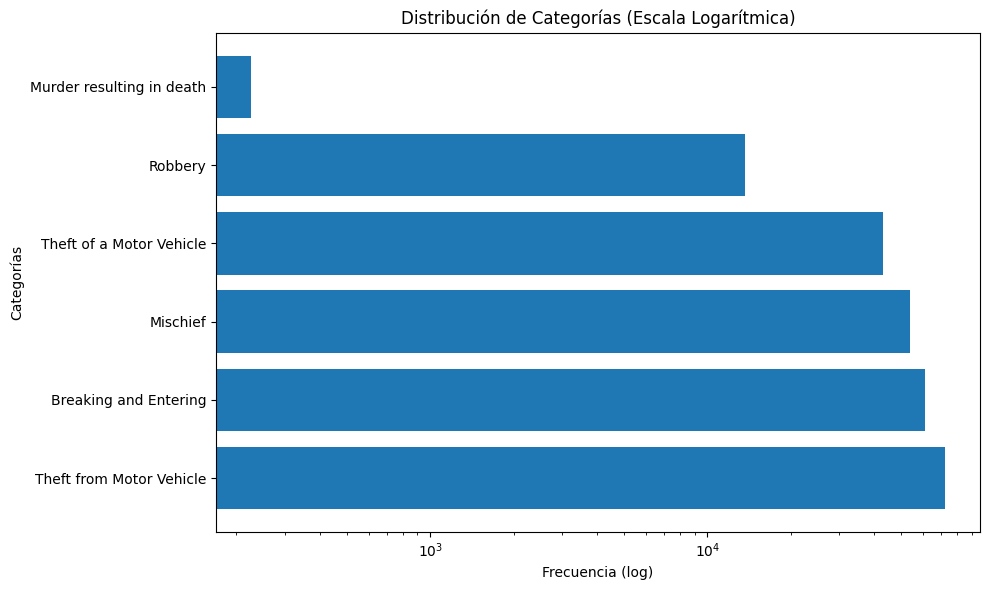
\includegraphics[width=0.85\linewidth]{../Imagenes/Reto_4/grafica_MayoresCrimenes.png}
            \caption{Comparativa de los crímenes más comunes en Montreal.}
            \label{fig:mayores_crimenes}
        \end{figure}
        Como se puede observar en la Figura \ref{fig:mayores_crimenes}, los tres crímenes más comunes en Montreal son: Robo de vehículo, ayanamiento de hogar (Breaking and Entering) y Mischief. Estos resultados indican que los delitos relacionados con la propiedad son predominantes en la ciudad, lo que sugiere la necesidad de fortalecer las medidas de seguridad y prevención en este ámbito.
    \item \textbf{¿A que horario del dia suceden la mayoria de incidentes?}
        Para responder esta pregunta, se realizó un análisis de frecuencia de la columna <<QUART>> en el conjunto de datos. Esto permitiendonos conocer el horario en el que suceden la criminalidad desde el 01 de Enero del 2015 hasta el 20 de Enero del 2023. Este análisis es fundamental para identificar los momentos del día en los que se concentran la mayoría de los incidentes criminales, lo que puede ser útil para la planificación de recursos policiales y la implementación de medidas de seguridad específicas durante esos periodos.
    \begin{figure}[H]
        \centering
            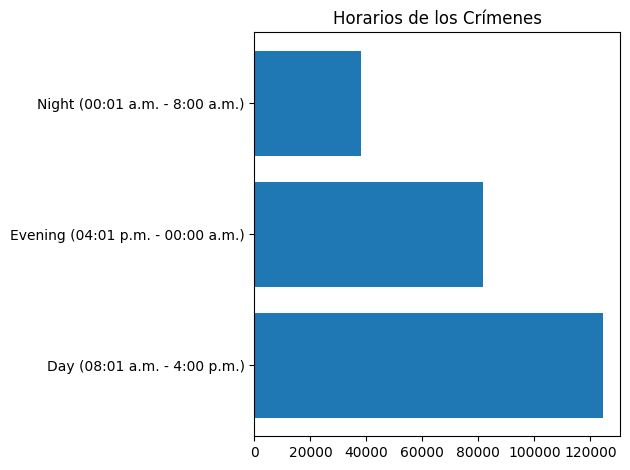
\includegraphics[width=0.85\linewidth]{../Imagenes/Reto_4/grafica_HorarioCrimenes.png}
            \caption{Comparativa del horario de los crímenes en Montreal.}
            \label{fig:horarios_crimenes}
        \end{figure}
        Como se puede observar en la Figura \ref{fig:horarios_crimenes}, el horario del día en el que se concentran la mayoría de los incidentes criminales es durante el dia. Este resultado sugiere que las actividades delictivas tienden a aumentar durante las horas mas activas de la ciudad, lo que puede estar relacionado con la mayor presencia de personas en espacios públicos y la mayor oportunidad para cometer delitos durante el día. Este hallazgo es importante para orientar las estrategias de prevención y patrullaje policial en los momentos del día en los que se registra una mayor incidencia de crímenes.
    \item \textbf{¿Cual de los 5 departamentos de policia (PDQ) tienen la mayor denuncia de delitos?}
        Para responder esta pregunta, se realizo un analisis de frecuencia de la columna <<PDQ>> en el conjunto de datos. Se identificaron los sectores policiales con mayor cantidad de denuncias de delitos, lo que permitió determinar cuál de los cinco departamentos de policía (PDQ) tiene la mayor incidencia de crímenes registrados. Este análisis es crucial para entender la distribución geográfica de la criminalidad en Montreal y para orientar las políticas de seguridad pública en las áreas más afectadas.
        \begin{figure}[H]
        \centering
            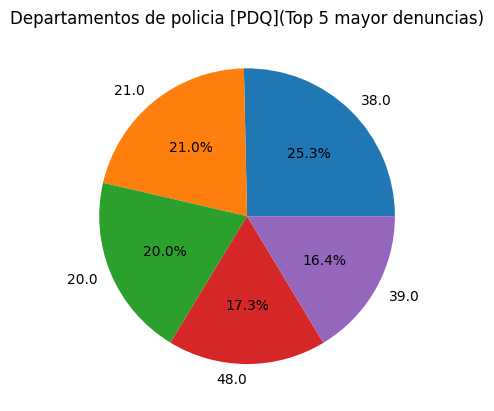
\includegraphics[width=0.85\linewidth]{../Imagenes/Reto_4/grafica_DepartamentosPolicias.png}
            \caption{Comparativa de los departamentos de policía con mayor denuncia de delitos en Montreal.}
            \label{fig:departamentos_MayorDenuncia}
        \end{figure}
        Como se puede observar en la Figura \ref{fig:departamentos_MayorDenuncia}, el departamento de policía (PDQ) con la mayor denuncia de delitos es el PDQ 38,21,20,48,39. Este resultado es importante para entender la distribución geográfica de la criminalidad en Montreal y para orientar las políticas de seguridad pública en las áreas más afectadas.
    \item \textbf{¿Cuales son los primeros 3 PDQs que tienen la menor denuncia de delitos?}
        Para responder esta pregunta, se realizó un análisis de frecuencia de la columna <<PDQ>> en el conjunto de datos. Se identificaron los sectores policiales con menor cantidad de denuncias de delitos, lo que permitió determinar cuáles son los tres departamentos de policía (PDQ) con la menor incidencia de crímenes registrados. Este análisis es crucial para entender las tendencias criminales y para orientar las políticas de seguridad pública en Montreal.
        \begin{figure}[H]
        \centering
            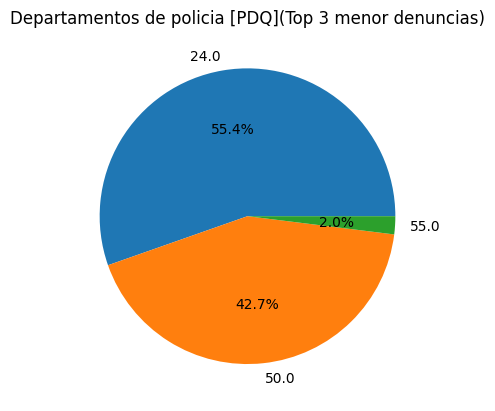
\includegraphics[width=0.85\linewidth]{../Imagenes/Reto_4/grafica_departamentoMenorDenuncia.png}
            \caption{Comparativa de los departamentos de policía con menor denuncia de delitos en Montreal.}
            \label{fig:departamentos_MenorDenuncia}
        \end{figure}
        Como se puede observar en la Figura \ref{fig:departamentos_MenorDenuncia}, los tres departamentos de policía (PDQ) con la menor denuncia de delitos son el PDQ 24, el PDQ 50 y el PDQ 55. Este resultado es importante para entender las tendencias criminales y para orientar las políticas de seguridad pública en Montreal, ya que puede indicar áreas con menor incidencia de crímenes o con una mayor eficacia en la prevención del delito.
    % \item \textbf{¿Que vecindario tiene el mayor registro de incidentes criminales y cuales son los tipos de crimenes en ese vecindario?}
    %     Para responder esta pregunta, se realizó un análisis de frecuencia de la columna <<PDQ>> en el conjunto de datos. Se identificaron los sectores policiales con mayor cantidad de denuncias de delitos, lo que permitió determinar cuál de los cinco departamentos de policía (PDQ) tiene la mayor incidencia de crímenes registrados. Este análisis es crucial para entender la distribución geográfica de la criminalidad en Montreal y para orientar las políticas de seguridad pública en las áreas más afectadas.
        
    %     \begin{figure}[H]
    %         \centering
    %         \begin{subfigure}[b]{0.8\textwidth}
    %             \centering
    %             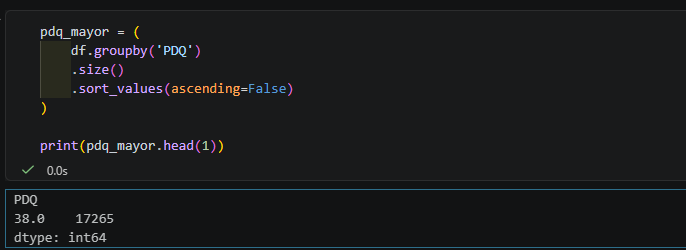
\includegraphics[width=\textwidth]{../Imagenes/Reto_4/PDQ_conMayorCriminalidad.png}
    %             \caption{PDQ con mayor registro de incidentes criminales.}
    %             % \label{fig:vecindario_MayorRegistro}
    %         \end{subfigure}
    %         \hfill
    %         \begin{subfigure}[b]{0.8\textwidth}
    %             \centering
    %             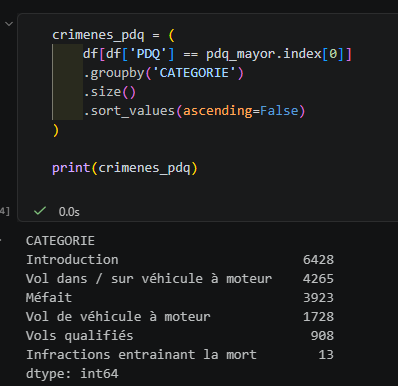
\includegraphics[width=\textwidth]{../Imagenes/Reto_4/criminalidad_enElPDQ.png}
    %             \caption{Consulta de criminalidad en el PDQ.}
    %             % \label{fig:K_Optimo}
    %         \end{subfigure}
    %     \end{figure}
    %     Como se puede observar en la Figura \ref{fig:vecindario_MayorRegistro}, los tres crímenes más comunes en Montreal son: Robo de vehículo, ayanamiento de hogar (Breaking and Entering) y Mischief. Estos resultados indican que los delitos relacionados con la propiedad son predominantes en la ciudad, lo que sugiere la necesidad de fortalecer las medidas de seguridad y prevención en este ámbito.
    \item \textbf{¿Qué vecindario tiene el mayor registro de incidentes criminales y cuáles son los tipos de crímenes presentes en ese vecindario?}

Para responder esta pregunta, se realizó un análisis de frecuencia de la columna <<PDQ>> en el conjunto de datos. Se identificaron los sectores policiales con mayor cantidad de denuncias de delitos, lo que permitió determinar cuál de los sectores policiales (PDQ) presenta la mayor incidencia de crímenes registrados. Este análisis es crucial para comprender la distribución geográfica de la criminalidad en Montreal y orientar las políticas de seguridad pública hacia las áreas más afectadas.

\begin{figure}[H]
    \centering

    \begin{subfigure}[b]{0.8\textwidth}
        \centering
        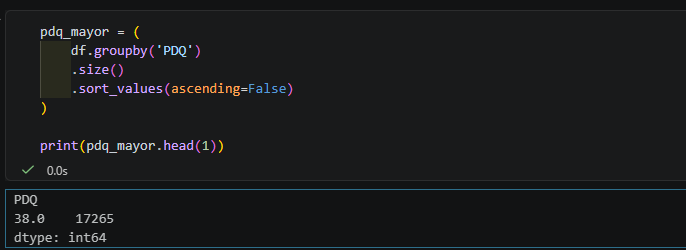
\includegraphics[width=\textwidth]{../Imagenes/Reto_4/PDQ_conMayorCriminalidad.png}
        \caption{PDQ con mayor registro de incidentes criminales.}
    \end{subfigure}

    \vspace{0.5cm}

    \begin{subfigure}[b]{0.8\textwidth}
        \centering
        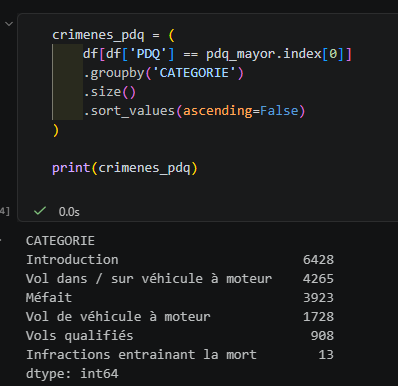
\includegraphics[width=\textwidth]{../Imagenes/Reto_4/criminalidad_enElPDQ.png}
        \caption{Distribución de criminalidad dentro del PDQ con mayor incidencia.}
    \end{subfigure}

    \caption{Análisis del sector policial con mayor incidencia criminal.}
    \label{fig:vecindario_MayorRegistro}
\end{figure}
El análisis realizado sobre la variable \texttt{PDQ} permitió identificar el sector policial con mayor concentración de incidentes criminales registrados en el conjunto de datos. Como se observa en la Figura (a), el PDQ 38 presenta el mayor número de reportes, acumulando un total de 17,265 incidentes criminales. Este resultado indica que dicho sector representa una de las zonas con mayor actividad delictiva dentro de la ciudad de Montreal.

Posteriormente, se realizó un análisis de frecuencia de los tipos de delitos registrados específicamente dentro del PDQ 38. Los resultados muestran que los crímenes predominantes corresponden a:

\begin{itemize}
\item \textbf{Introduction} (allanamiento de hogar): 6,428 incidentes.
\item \textbf{Vol dans / sur véhicule à moteur} (robo dentro o sobre vehículo): 4,265 incidentes.
\item \textbf{Méfait} (vandalismo o daños a propiedad): 3,923 incidentes.
\end{itemize}

En menor proporción también se registraron delitos como:
\begin{itemize}
\item Robo de vehículo.
\item Robo con violencia.
\item Delitos que derivaron en muerte.
\end{itemize}

Estos resultados evidencian que los delitos patrimoniales representan la principal problemática criminal dentro del PDQ analizado. La alta frecuencia de allanamientos y robos relacionados con vehículos sugiere una fuerte incidencia de delitos contra la propiedad privada, lo cual puede estar asociado a factores urbanos, densidad poblacional o actividad económica de la zona.

Asimismo, la baja frecuencia de delitos relacionados con homicidios indica que, aunque existen incidentes de alta gravedad, estos ocurren con mucha menor frecuencia en comparación con los delitos patrimoniales. En términos generales, el análisis permite concluir que la criminalidad en el PDQ 38 se encuentra dominada principalmente por delitos no violentos relacionados con bienes materiales y afectaciones a la propiedad.
    \item \textbf{¿Cual vecindario es el que tiene mayor casos de asesinato?}
        Para responder esta pregunta, se realizó un análisis de frecuencia de la columna <<CATEGORIE>> en el conjunto de datos. Se identificaron los tipos de crímenes más comunes registrados en la ciudad, lo que permitió determinar cuáles son los tres crímenes más relevantes u ofensas cometidas. Este análisis es crucial para entender las tendencias criminales y para orientar las políticas de seguridad pública en Montreal.
        \begin{figure}[H]
        \centering
            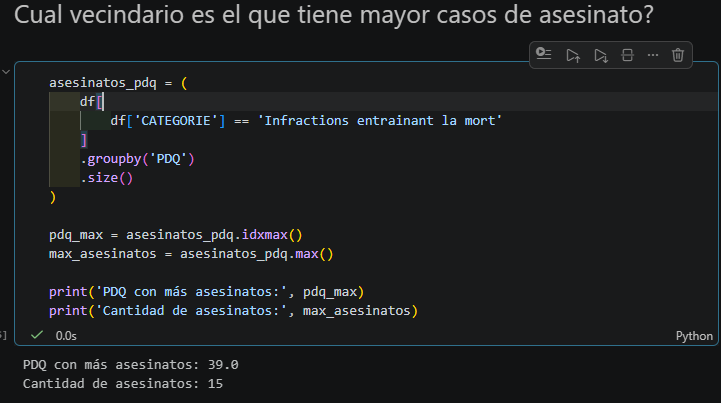
\includegraphics[width=0.85\linewidth]{../Imagenes/Reto_4/PDQ_mayorAsesinatos.png}
            \caption{Comparativa de los crímenes más comunes en Montreal.}
            \label{fig:vecindario_MayorAsesinatos}
        \end{figure}
        Como se puede observar en la Figura \ref{fig:vecindario_MayorAsesinatos}, el vecindario con mayor casos de asesinato es el PDQ 39. Este resultado indica que dicho sector representa una de las zonas con mayor actividad delictiva dentro de la ciudad de Montreal, específicamente en relación a los delitos de homicidio. Este hallazgo es importante para orientar las políticas de seguridad pública y las estrategias de prevención del delito en esa área específica.
\end{enumerate}

\subsection{HeatMap}

Como complemento al análisis, se incorporó un mapa geográfico junto con un HeatMap con el objetivo de representar visualmente la distribución espacial de la criminalidad en Montreal.

Además, al interactuar con el mapa, es posible visualizar un \textit{tooltip} que muestra información relacionada con el tipo de crimen y la cantidad de incidentes registrados en cada zona. Esto facilita la interpretación de la información geoespacial y permite identificar patrones o tendencias delictivas de manera más intuitiva.
\begin{figure}[H]
    \centering
    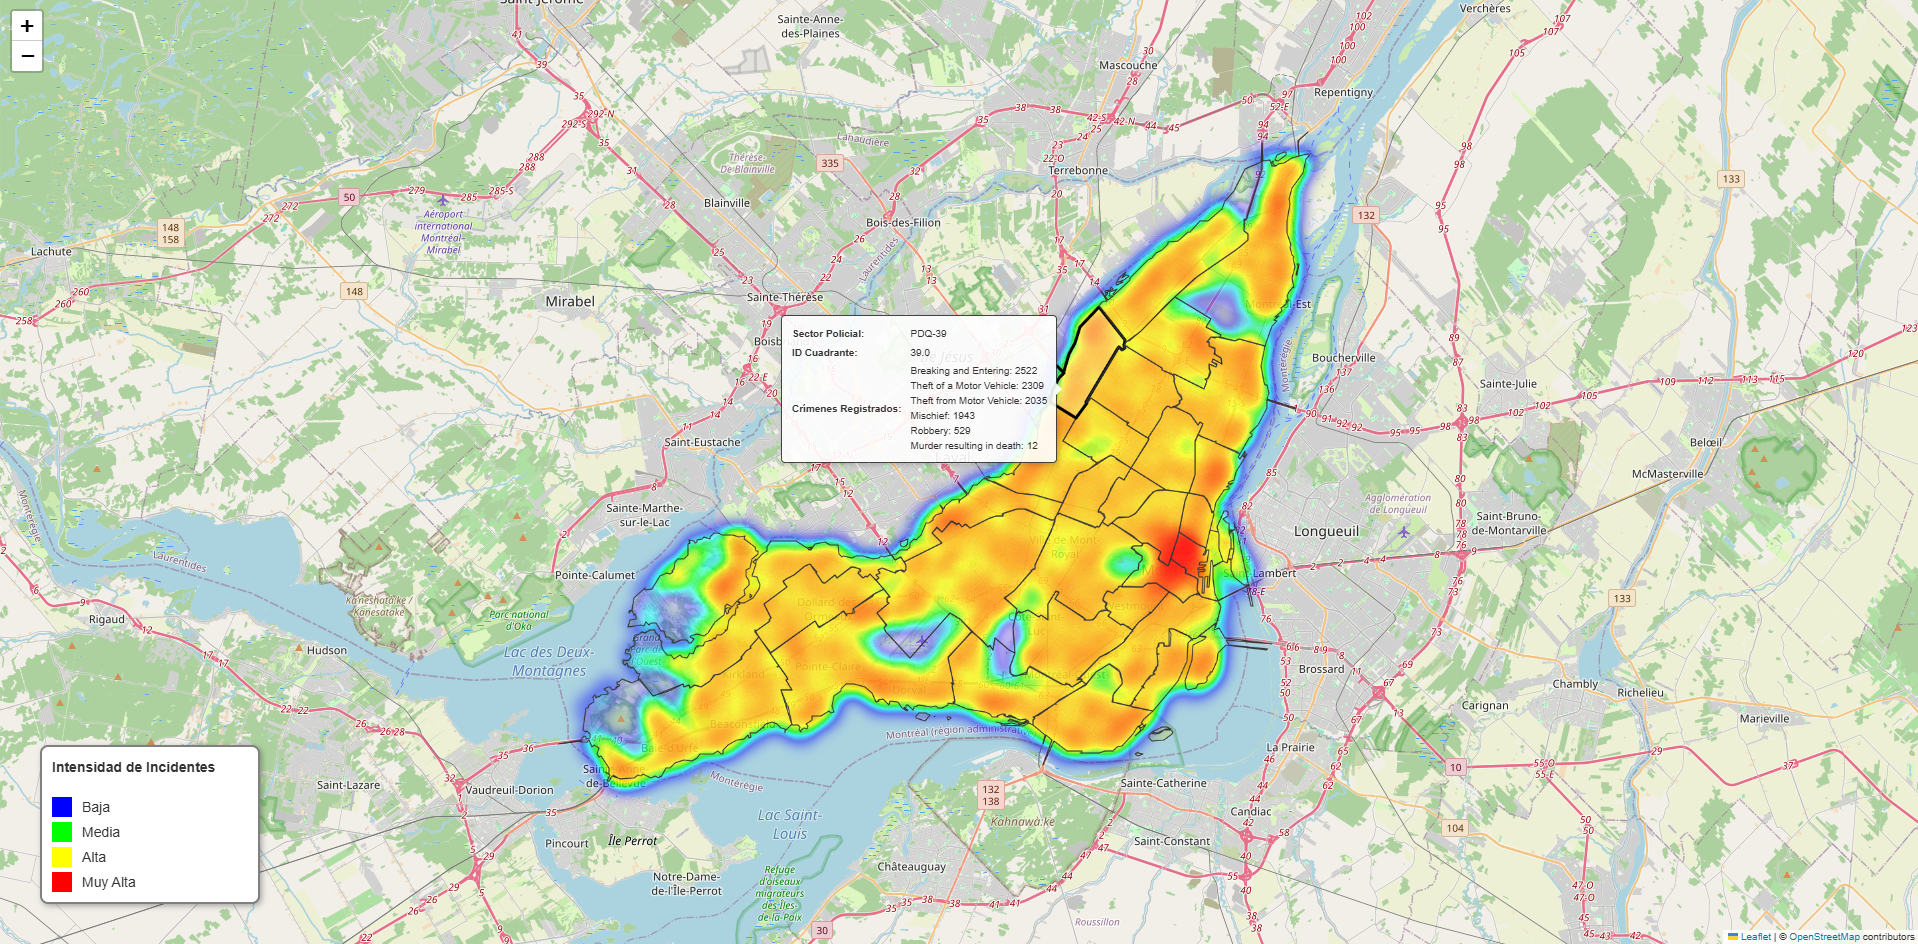
\includegraphics[width=0.85\linewidth]{../Imagenes/Reto_4/Mapa_Criminalidad.png}
    \caption{Mapa geográfico con HeatMap de criminalidad en Montreal.}
    \label{fig:mapa_criminalidad}
\end{figure}


\section{Conclusión}

A través del desarrollo del presente proyecto fue posible aplicar distintas técnicas de análisis y visualización de datos para estudiar el comportamiento criminal en la ciudad de Montreal. Mediante el uso de herramientas de ciencia de datos en Python, se logró transformar y analizar un conjunto de datos geoespaciales con información criminal correspondiente al periodo 2015--2023.

Los resultados obtenidos permitieron identificar que los delitos relacionados con la propiedad, como el robo de vehículos, allanamientos y actos de vandalismo, representan la mayor proporción de incidentes criminales registrados en la ciudad. Asimismo, se observó que ciertos sectores policiales (PDQ) presentan concentraciones significativamente mayores de actividad delictiva, destacando particularmente el PDQ 38 como una de las zonas con mayor número de incidentes reportados.

De igual manera, el análisis temporal mostró que la mayoría de los crímenes ocurren durante el día, mientras que el análisis geoespacial mediante mapas de calor permitió visualizar las zonas urbanas con mayor densidad criminal. Estos hallazgos evidencian la utilidad de las técnicas de visualización geográfica para apoyar el análisis de fenómenos urbanos complejos.

Finalmente, el proyecto permitió reforzar conocimientos relacionados con limpieza de datos, análisis exploratorio, agrupación estadística y representación geoespacial de información. Además, demuestra cómo las herramientas de análisis de datos pueden contribuir al entendimiento de problemáticas sociales y servir como apoyo para la toma de decisiones en materia de seguridad pública.
\printbibliography[title={ Bibliográfia}]
\end{document}